\chapter[Plaquette-MIDO]{Plaquette-MIDO\raisebox{.3\baselineskip}{\normalsize\footnotemark}}
\footnotetext{\url{https://github.com/Dauphine-MIDO/plaquette-MIDO}}

Ce projet a pour but d'implémenter un code générant un fichier PDF détaillant les différents enseignements du Master 1 MIAGE en apprentissage à partir de la base de données de Dauphine. La finalité est d'automatiser le lancement du code du sorte que quotidiennement le fichier PDF soit mis à jour et publié en ligne.

À mon arrivée, un code permettait déjà la génération du fichier PDF. Certains passages du code était cependant à revoir pour améliorer l'esthétique du fichier PDF. De plus, le code initial était très peu généralisé à d'autres utilisateurs et plusieurs changements dans le code était nécessaire pour qu'un autre utilisateur puisse lancer Plaquette-MIDO. Il fallait donc davantage généraliser le code de façon à rendre accessible le code à d'autres utilisateurs. Le principal aspect à généraliser était l'authentification à l'API de Dauphine, indispensable pour avoir accès aux données de l'université.

\section{L'authentification}

Pour se connecter à l'API de Dauphine, un nom d'utilisateur et un mot de passe sont nécessaires. Le code initial prévoyait trois manières différentes de fournir ces informations afin de se connecter à l'API :
\begin{itemize}
    \item les propriétés du système
    \item les variables d'environnement
    \item un fichier texte contenant les informations nécessaires
\end{itemize}

Seulement, ce code ne lisait initialement que le mot de passe et le nom d'utilisateur était une valeur par défaut. Un nouvel utilisateur devait donc modifier le code pour pouvoir utiliser ses identifiants. L'idée d'une valeur par défaut pour le nom d'utilisateur a donc abandonné pour rendre le programme plus accessible. La valeur du nom d'utilisateur serait lue de la même manière que celle du mot de passe.

\subsection{La classe Authentication}

Une nouvelle classe a donc été créée pour permettre la généralisation lecture du code et améliorer sa lisibilité. Celle-ci permet de créer un objet contenant un nom d'utilisateur et un mot de passe de type Optional. Ce type permet d'instancer aussi bien la valeur d'une chaîne de caractère que l'absence d'une information. Il permet ainsi de 

\subsection{Le projet CredsRead}
La généralisation du code permettant l'authentification nous a poussé à le séparer dans un projet bien distinct de Plaquette-MIDO, le projet CredsRead. Celui-ci sera ensuite intégré au code source de Plaquette-MIDO.

\section{L'automatisation du lancement du code}

La finalité du projet Plaquette-MIDO est de lancer la construction du fichier PDF quotidiennement et de le publier de manière à ce qu'il soit accessible sur le site de Dauphine. Pour réaliser cette automatisation, j'ai utilisé l'outil Travis-CI.

\subsection{Travis-CI}
    Travis-CI est logiciel d'intégration continue qui permet de compiler,
    tester et déployer le code de dépôts GitHub. Il est configurer à partir
    d'un fichier nommé \texttt{.travis.yml} présent dans la racine du
    répertoire. Celui-ci est lu à chaque nouveau commit par Travis-CI qui
    exécute son contenu sur une machine virtuelle. L'exécution peut alors
    réussir dans le cas où aucune erreur n'a été signalée ou échouer si une
    erreur est survenue. Travis-CI peut donc s'assurer de la bonne
    compilation d'un projet. Il peut également effectuer des déploiements.
    En effet, il est possible d'insérer du script que Travis-CI exécute pour
    déployer des fichiers. Par exemple, ajouter un script avec les commandes
    git adéquat pour pousser des fichiers vers un dépôt. Travis-CI peut donc
    exécuter le code source permettant la création du fichier PDF et ensuite
    déployer ce fichier vers un dépôt GitHub.

\begin{figure}[!h]
    \begin{center}
    %taille de l'image en largeur
    %remplacer "width" par "height" pour régler la hauteur
    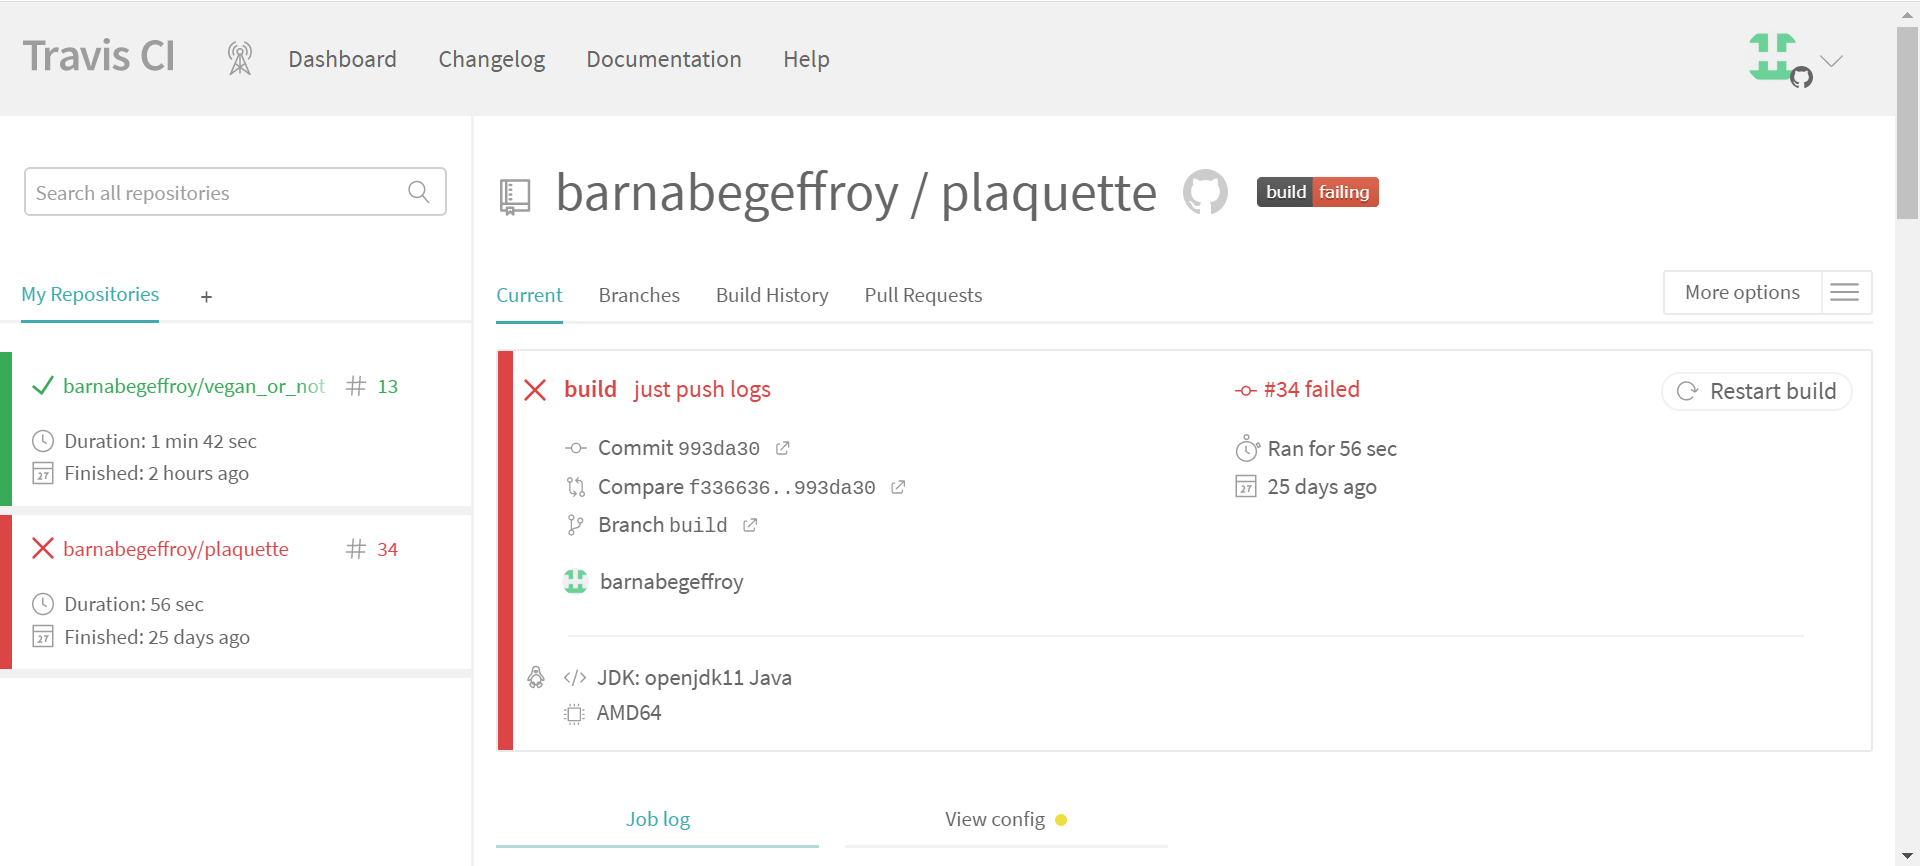
\includegraphics[width=13cm]{assets/travis-ci.PNG}
    \end{center}
    %légende de l'image
    \caption{Enveloppe d'un son}
\end{figure}


Travis-CI permet également de référencer des variables d'environnement sécurisées (clefs d'accès, identifiants,...)
\begin{figure}[!h]
    \begin{center}
    %taille de l'image en largeur
    %remplacer "width" par "height" pour régler la hauteur
    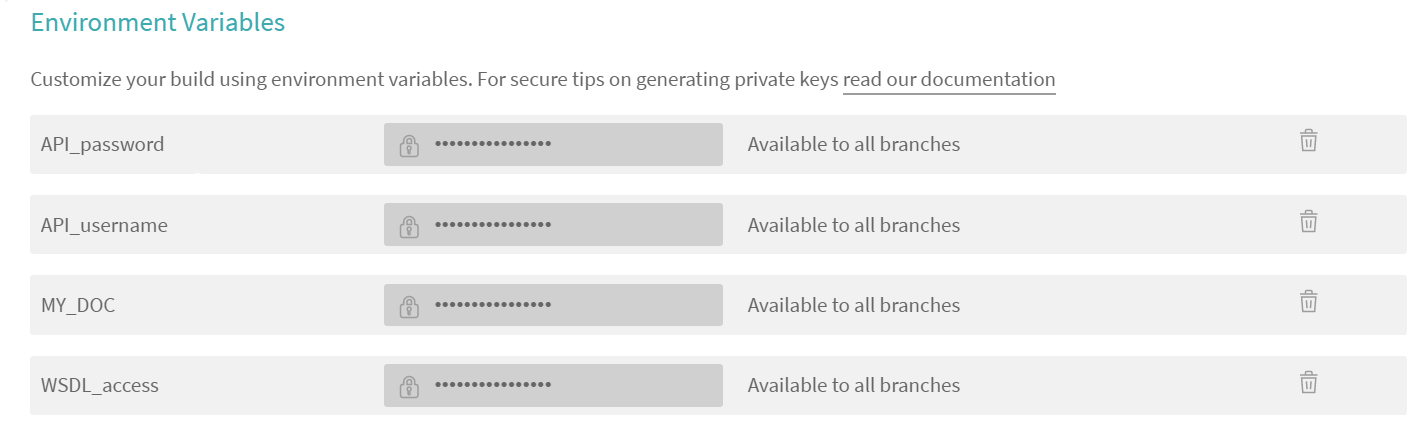
\includegraphics[width=13cm]{assets/env.PNG}
    \end{center}
    %légende de l'image
    \caption{Enveloppe d'un son}
\end{figure}

\subsection{L'exécution du code}
\subsubsection*{Les dépendances}



Travis-CI identifie automatiquement un projet Maven et installe les dépendances indiquées dans le \texttt{pom.xml}. Dans le projet Plaquette-MIDO, la dépendance qui importe le code source de l'API de Dauphine nécessite un fichier texte nommé \texttt{WSDL\_Login.txt} contenant un URL spécifique des identifiants de l'utilisateur. Ce fichier ne peut pas être dans le dépôt car il contient des informations personnelles. Il faut donc un script qui crée le fichier sur la machine virtuelle de Travis-CI. Avant de lancer l'installation des dépendances le fichier doit donc être créer. Dans le \texttt{.travis.yml}, on peut ajouter un script qui génère ce fichier.

\subsubsection*{Création du fichier PDF et déploiement}
Une fois que toutes les dépendances du projet Maven sont installées, il faut executé le code source qui génère le fichier PDF. La méthode main a executé se trouve dans la classe \texttt{M1ApprBuilder.java}. Le déploiement vers le dépôt d'arrivée doit également être pris en compte. Voici le script exécuté par Travis-CI pour réaliser ce travail :


\subsubsection*{Automatisation}
Travis-CI lance initiallement la construction du code à chaque nouveau commit. Il est cependant possible de configurer des \textit{Cron Jobs}. Ceux-ci vont renouveler la construction du code de manière quotidienne, hebdomadaire ou mensuelle. 

\begin{figure}[!h]
    \begin{center}
    %taille de l'image en largeur
    %remplacer "width" par "height" pour régler la hauteur
    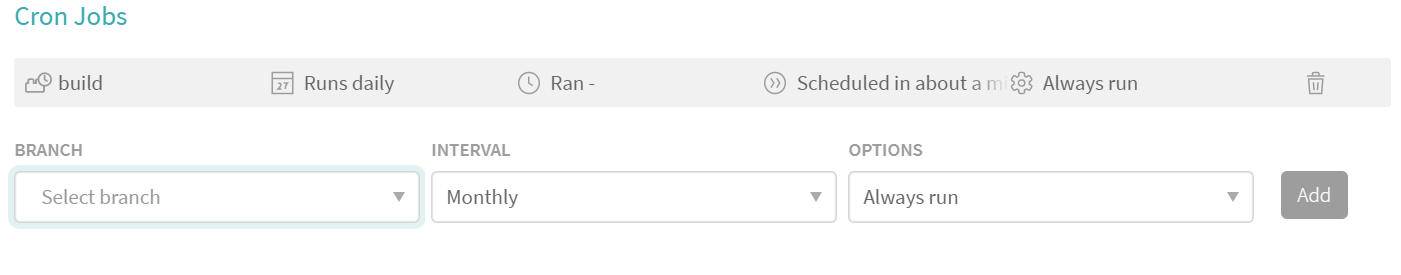
\includegraphics[width=13cm]{assets/CronJobs.PNG}
    \end{center}
    %légende de l'image
    \caption{Enveloppe d'un son}
\end{figure}

En programmant sur \textit{Daily}, Travis-CI va relancer la construction du code tous les jours et ainsi renouveller le fichier PDF et les logs si des changements sont effectués. Si une erreur se produit et que le fichier PDF n'est pas généré, une e-mail nous previendra de la non-construction du code et le fichier PDF le plus récent sera toujours disponible sur le site.